\subsection{Motivation}
The paradigmatic problem of Fast Multipole Methods (\textbf{\gls{FMM}})
\footnote{The first usage of a technical term or abbreviation listed in the
glossary is highlighted throughout the text for ease of reference.} is the so
called $N$-Body problem. This classic problem refers to the calculation of the pairwise
interactions between $N$ particles over a potentially long-range, for example in
gravitational or electrostatic problems. The straightforward calculation can be
written in the form of the following sum,

\begin{equation}
\Phi(x_j) = \sum_{i=1}^N w_i K(x_i, x_j)
\label{eq:n_body_problem}
\end{equation}

Where $i, j \in [1,N]$ and $K(x, y)$ is called the Green's function, or equivalently
a `kernel function', where one is generally concerned with coordinates of particles in an
$n=2 \> \> \text{or} \> \> 3$ dimensional Hilbert space taking  $\ x_i \in \mathbb{R}^n$.
Additionally, each summand is weighted by $w_i$. For solving for electrostatic
potential in three dimensions, which is used as the model problem throughout this
thesis, this goes to,

\begin{equation}
\Phi(x_j) = \sum_{i=1}^N q_iK(x_i, x_j)
\label{eq:electrostatic_paradigm}
\end{equation}

where $q_i$ refers to a charge density with the kernel function,

\begin{equation}
    K(x, y) = \frac{1}{4\pi \epsilon_0}\frac{1}{| x - y |}
\label{eq:laplace_kernel}
\end{equation}

the constant $\epsilon_0$ is the permittivity of free space. It's easy to see
how a naive direct application of this equation over $N$ particles
results in an algorithm of $O(N^2)$ complexity, therefore it's only practicable
for systems of moderate size, whereas in realistic systems, one may be interested in
interactions involving $10^{6}$ to $10^8$ particles.

This chapter introduces the analytic \gls{FMM}, the kernel-independent
version, which is the main focus of this thesis, is presented later.
Though substantially different in implementation, the analytic FMM will provide the opportunity
to exposit many of the key ideas behind all FMM-based algorithms, and provides
a good starting point for understanding and developing upon these algorithms.
First presented by Greengard \cite{Greengard:1987:Yale},
the analytic \gls{FMM} represented a sea change for $N$-Body simulation. By
trading off computations for error, it manages to achieve an asymptotic complexity
 of just $O(N)$. Additionally, it comes equipped with rigorous error bounds,
making fast and accurate massive $N$-Body simulations feasible on available
computing hardware. It's success has been such that it is regarded as one of
the key developments in numerical algorithms in the twentieth century \cite{Cipra:2000:SN}.

The original analytic FMM solves the electrostatic problem
in two and three dimensions, this is equivalently known as the Poisson problem,
represented by the differential equation,

\begin{equation}
    \nabla^2 \phi =f
\label{eq:poisson}
\end{equation}

Where $\phi$ is some scalar potential to be determined, and $f$ is a scalar source
term which is usually known. For electrostatics the corresponding formulation
can be derived from Gauss' law as \cite{Griffiths:2017:CUP},

\begin{equation}
  \nabla^2 \phi = - \frac{q}{\epsilon_0}
\label{eq:electrostatic_poisson}
\end{equation}

where $\phi$ is the electrostatic potential, $q$ is the charge density and
$\epsilon_0$ is the permittivity of free space. It can therefore be seen that
the \gls{FMM} is actually solving the Poisson problem by reformulating it as an
integral equation. The ubiquity of problems of the form (\ref{eq:n_body_problem})
in computational science has lead to diverse application of the FMM. For example,
in the modeling the electrostatic interactions of charged particles in complex
biological molecules at biologically relevant length scales \cite{Board:1992:CPL}.
The extension of FMMs to Helmholtz equations \cite{Rokhlin:1990:JCP}, has lead
to even more applications, such as in seismic and acoustic scattering
\cite{Hwu:2011:MKP}. Though as the focus of this thesis is on solving the Poisson
model problem for electrostatics, this is mentioned only for completeness.

The key insight that leads to the \gls{FMM}'s asymptotic complexity is the idea
that if the field created by a distribution of charge (or mass) density is approximated
to be relatively smooth in the \textbf{\gls{far-field}}, then it should be possible to apply
some form of compression for the evaluation of contribution to local potentials due
to particles in the \gls{far-field}. The FMM performs this compression by encoding
the field contributions of particles in the \gls{far-field} using a multipole
expansion.

For simple kernel functions and charge distributions, such as the model problem
of this thesis, one can easily derive the expression for this multipole expansion
by finding an series expansion of the system's Green's function.
In order to generalise the discussion, an arbitrary continuous
distribution of charge is considered as shown in figure \ref{fig:1_1_continuous_charge_distribution},
for which the potential is evaluated at some other evaluation point outside of
the distribution. This can be written as follows \cite{Griffiths:2017:CUP},

\begin{flalign}
    \Phi(\mathbf{r}) = \frac{1}{4 \pi \epsilon_0} \int \frac{1}{d}\rho(\mathbf{r}')d\tau'
    \label{eq:1_1_continuous_integral_formulation}
\end{flalign}

where $\rho(\mathbf{r}')$ is a charge density, and the other symbols take their
meanings from figure (\ref{fig:1_1_continuous_charge_distribution}).


\begin{figure}[!h]
    \centering
    {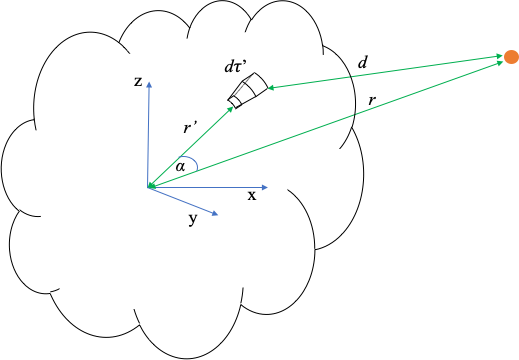
\includegraphics[width=0.45\textwidth]{introduction/continuous_charge.png}}
  \vspace{0pt}
  \caption{An arbitrary charge distribution, with an orange point to mark a point
  where the potential is being evaluated. Here, $\mathbf{r}$ is the the vector
  between the centre of the multipole expansion and the evaluation point, $\mathbf{r}'$
  is the vector between the centre of expansion and a given volume element $d\tau'$, and
  $d$ is a vector between the volume element $d\tau'$ and the evaluation point.}
  \label{fig:1_1_continuous_charge_distribution}
\end{figure}

From law of the cosines,

\begin{flalign}
    d^2 &= r^2 + (r')^2 - 2rr'\cos \alpha = r^2 \left [ 1 + \left ( \frac{r'}{r} \right)^2 - 2 \left (\frac{r'}{r} \right)\cos \alpha \right]\\
    d &= r \sqrt{1+\epsilon}
    \label{eq:1_1_law_of_cosines}
\end{flalign}

Where,

\begin{flalign}
    \epsilon \equiv \left ( \frac{r'}{r} \right) \left (\frac{r'}{r} - 2 \cos \alpha \right)
\end{flalign}

As $\epsilon$ is small far away from charge distribution one can expand $1/d$ binomially,

\begin{flalign}
    \frac{1}{d} &= \frac{1}{r}(1+\epsilon)^{-1/2} = \frac{1}{r}\left (1 - \frac{1}{2}\epsilon + \frac{3}{8}\epsilon^2 - ... \right) \\
    \frac{1}{d} &= \frac{1}{r} \sum_{n=0}^{\infty} \left(\frac{r'}{r} \right)^n P_n(\cos \alpha)
\end{flalign}

Using this, the exact multipole expansion for this charge distribution is,

\begin{flalign}
    \Phi(\mathbf{r}) = \frac{1}{4 \pi \epsilon_0}\sum_{n=0}^{\infty}\frac{1}{r^{n+1}}\int (r')^nP_n(\cos \alpha)\rho(\mathbf{r'}) d \tau'
\end{flalign}

If instead one considers a charge distribution composed of $N$ discrete charges
$q_i$ this goes to,

\begin{flalign}
    \Phi(\mathbf{r}) = \frac{1}{4 \pi \epsilon_0}\sum_{i=1}^N\sum_{n=0}^{\infty}\frac{(r')^n q_i}{r^{n+1}}P_n(\cos \alpha)
\end{flalign}

Using the addition theorem for Legendre polynomials \cite{Greengard:1987:Yale},

\begin{flalign}
    P_n(\cos \gamma) = \sum_{m=-n}^n Y_n^{-m}(\alpha, \beta) Y_n^m(\theta, \phi)
\end{flalign}

Where the Legendre polynomial is written in terms of spherical harmonics,
where $(r, \theta, \phi)$ and $(\rho, \alpha, \beta)$ define two spherical coordinates,
and $\gamma$ is the angle subtended between them. Therefore, the multipole expansion goes to,

\begin{flalign}
    \Phi(\mathbf{r}) &= \frac{1}{4 \pi \epsilon_0}\sum_{i=1}^N\sum_{n=0}^{\infty}\frac{(r')^n q_i}{r^{n+1}}P_n(\cos \alpha)\\
    & = \frac{1}{4 \pi \epsilon_0}\sum_{i=1}^N\sum_{n=0}^{\infty}\sum_{m=-n}^n \frac{(r')^n q_i Y_n^{-m}(\alpha_i, \beta_i) }{r^{n+1}}Y_n^m(\theta, \phi)\\
    & = \sum_{i=1}^N\sum_{n=0}^{\infty}\sum_{m=-n}^n\frac{M_n^m}{r^{n+1}} \cdot Y_n^m(\theta, \phi)
    \label{eq:1_1_multipole_expansion}
\end{flalign}

This is an exact expansion, and it converges for $\frac{r'}{r} < 1$. This convergence
condition means that estimating of the potential at a given evaluation point
calculated using the multipole expansion is only possible in the far-field, the
boundary of which is often tuned empirically for different systems as it's user
defined. If instead the expansion is taken with centre at the evaluation point,
one can rewrite as the multipole expansion as a `local' expansion,

\begin{flalign}
    \Phi(\mathbf{r}) & = \frac{1}{4 \pi \epsilon_0}\sum_{i=1}^N\sum_{n=0}^{\infty}\sum_{m=-n}^n \frac{(r)^n q_i Y_n^{-m}(\alpha_i, \beta_i) }{r'^{n+1}}Y_n^m(\theta, \phi)\\
    & = \frac{1}{4 \pi \epsilon_0} \sum_{i=1}^N \sum_{n=0}^{\infty} \sum_{m=-j}^n L_m^n \cdot  Y_m^n(\theta, \phi) \cdot r^j
    \label{eq:1_1_local_expansion}
\end{flalign}

which converges when $\frac{r}{r'} < 1$. The region of convergence for both types
of expansions are shown in figure (\ref{fig:1_1_multipole_local_expansions}).

The key point to note is that the multipole and local expansions are exact, and
can be truncated as required to ensure that the asymptotic complexity of evaluating
a multipole or local expansion at an evaluation point is bounded by $O(N)$. A
rigorous error analysis of the analytic FMM is outside the scope of this thesis, and
we defer to the literature for exact expressions for these truncation errors \cite{Greengard:1987:Yale},
Furthermore, exact operations exist for shifting the center of these expansions,
as well as translating multipole expansion coefficients into equivalent local expansion
coefficients,
which are crucial in providing the improvements to asymptotic complexity\footnote{
    Expressions for these shift operators for the three dimensional Laplace kernel
    considered as our model problem are provided in Appendix \ref{app:3d_laplace}.
}.

\begin{figure}[!h]
    \centering
    {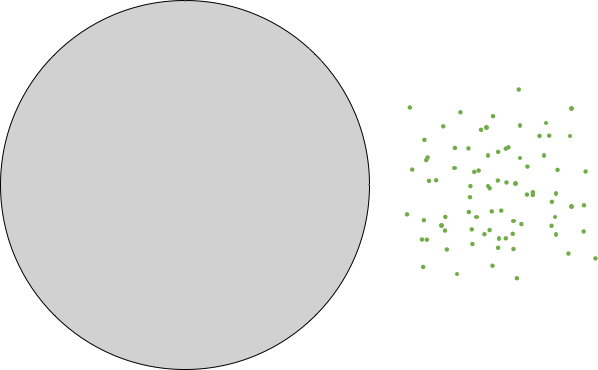
\includegraphics[width=0.33\textwidth]{introduction/multipole_expansion.png}}
    \hfill
  {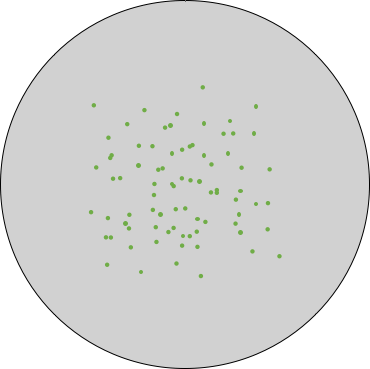
\includegraphics[width=0.4\textwidth]{introduction/local_expansion.png}}
  \vspace{0pt}
  \caption{(A) A multipole expansion centered on charge distribution. (B) A local
  expansion, centered around a point of evaluation. Regions in which the expansions
  converge are shaded in grey. For the multipole expansion this is the entire domain
  outside of the region for $r>r'$, and for the local expansion this is the region
  for which $r < r'$}

  \label{fig:1_1_multipole_local_expansions}
\end{figure}

\hspace{10pt}

\subsection{Algorithm Structure \& Analysis}

The convergence condition of the multipole expansion prohibits the compression
of charges from particles in the \textbf{\gls{near-field}}. Therefore the FMM
makes use of a tree structure in a recursive algorithm, this structure is known
as an Octree in three dimensions and a Quadtree in two dimensions\footnote{The usage
of trees naturally leads to biological adjectives to describe it's structure, for example
the coarsest level of a tree is referred to as the `root' level, and the finest
level as the `leaf' level.}. This structure
hierarchically partitions space such that each level, $l$, of the tree is equally partioned into
$(2^d)^l$ boxes\footnote{Regardless of the spatial dimension, partitions of a domain are invariably
referred to as boxes.} over the domain of the tree, where $d$ is the dimension,
i.e. $d=3$ in three dimensions. If one were to simply traverse the tree from
the coarsest, or `root', level to the finest, or `leaf', level and find the multipole expansion of source
particles in each box of each level, one could then evaluate these multipole expansions
at each particle to solve the $N$-Body problem. As there are $O(\log(N))$
boxes in the tree, and $N$ particles this results in a $O(N\log(N))$ asymptotic
complexity.

However the FMM reduces computational complexity further by making use of local
expansions. Using the exact expressions to shift the multipole expansion
coefficients\footnote{Expressions for these shift operators for the three dimensional
Laplace kernel considered as our model problem are provided in Appendix \ref{app:3d_laplace}.}
$M_n^m$ to local expansion coefficients $L_n^m$ one can approximate the the interaction
between two boxes in the tree. Roughly speaking, because of the hierarchical
nature of the tree, each box only needs to consider the interaction with a
constant number of neighbouring boxes. Because the number of boxes $O(N)$,
the FMM is bound by an $O(N)$ asymptotic complexity \cite{Hwu:2011:MKP}.

Using the above analysis, one can then describe the FMM algorithm in terms of
two basic steps,

\begin{enumerate}
    \item \textbf{\textit{Upward Pass}}: The tree is traversed \textbf{\gls{post-order}}.
    Beginning at the leaf boxes, a multipole expansion is computed for each box
    due to the \textbf{\gls{source-particles}} it contains. This is also referred to as the particle-to-multipole
    operation, or \textbf{\gls{P2M}}. Then as one moves up the tree hierarchy, the
    multipole expansions of a each box's parent box is computed by shifting the
    expansion centers of the multipole expansion of a given child box, to the center
    of the parent box a, in a multipole-to-multipole operation or \textbf{\gls{M2M}},
    and summing together all the coefficients. Following the upward pass, one
    obtains the multipole expansion for each box containing source particles at
    all levels of the hierarchical tree.
    \item \textbf{\textit{Downward Pass}}: The tree is now traversed in
    \textbf{\gls{pre-order}}, and the local expansion of each box is computed.
    This local expansion is the sum of two parts: (1) the local expansion of the
    parent box of a given box, if it exists, which is a compression of the potential due to boxes
    non-adjacent to a given box's parent. The parent box's local expansion centre
    is shifted to the center of the child box, this is also known as the local-to-local
    operation or \textbf{\gls{L2L}}. (2) The multipole expansion of boxes which
    are the children of the \textbf{\gls{near-neighbours}} of a given box's
    parent but are not adjacent to the box itself. Such `source' boxes are described
    as being in the \textbf{\gls{interaction-list}} of a given box. These multipole
    expansions for each source box in a given box's interaction list are translated into local expansions centered at
    the given box, this is also known as
    the multipole-to-local operation, or \textbf{\gls{M2L}}. Notice that the
    \gls{M2L} operation is only available from $l=2$ of the tree, as in coarser
    levels the \gls{interaction-list} for all boxes is empty. The coefficients found
    from (1) and (2) are summed for each box. Steps (1) and (2) are repeated for each
    box until the leaf level. At this point, the local expansion
    of each leaf box is evaluated at all the \textbf{\gls{target-particles}} it contains.
    This local-to-particle, or \textbf{\gls{L2P}}, operation encodes all the \gls{far-field}
    interaction of the target particles in this leaf box. This is then combined with
    a \gls{near-field} interaction, due to the source particles in the leaf box,
    as well as in the \gls{near-neighbours}, which are computed directly. As the
    tree is refined to the point where the leaf levels contain only a small constant
    number of particles, this final direct computation is of low cost.
\end{enumerate}


With this specification, a more detailed analysis of the algorithm is possible,
though we defer to \cite{Greengard:1987:Yale} for a rigorous discussion.
Firstly, as mentioned above, the tree must be refined such that the leaf boxes
contain only a small constant number of particles, $\kappa$. The level of refinement $n$
is therefore approximately taken to be $n \approx \log(N)$, where $N$ is the number
of \gls{source-particles} in the tree. Beginning with upward pass, at the leaf level each particle contributes to one
multipole expansion. If this expansion is truncated to contain $p$ multipole terms, the
\gls{P2M} operation has a complexity of $O(Np^2)$, which can be seen from
(\ref{eq:1_1_multipole_expansion}), as well as the fact that the nature of a
hierarchical tree means that are $O(N)$ boxes at the leaf level. The shift operators\footnote{
    Expressions for these shift operators for the three dimensional Laplace kernel
    considered as our model problem are provided in Appendix \ref{app:3d_laplace}
} \gls{M2L}, \gls{L2L} and \gls{M2M} require $p^4$ operations with this truncation,
so the computation of all of these are bounded by\footnote{A more precise
bound depends on the size of a given box's \gls{interaction-list}.} $O(Np^4)$. Finally,
evaluating the $p^{th}$ degree local expansions at each target particle in the
\gls{L2P} operation, is bounded by $O(Np^2)$. The choice for level of refinement
$n$, leads to $O(\kappa N)$ complexity for direct calculations at the
leaf level. The whole algorithm is therefore bounded by $O(N)$.
In practice, the number of expansion terms $p$ is chosen for a prescribed relative error $\epsilon$, using
\footnote{There are optimal choices for $c$, with the authors of \cite{Ying:2004:JCP}
specifying $c=\frac{4-\sqrt{3}}{\sqrt{3}}$ for three dimensional problems.}
$p=\log_c \epsilon$. The algorithm is illustrated in figure (\ref{fig:1_1_main_loop})
in the two dimensional case, which is direct analogue of the three dimensional case
which is the focus of this thesis, and a full pseudo-code specification is
provided in Appendix \ref{app:analytic_fmm}.

\begin{figure}[!h]
    \centering
    {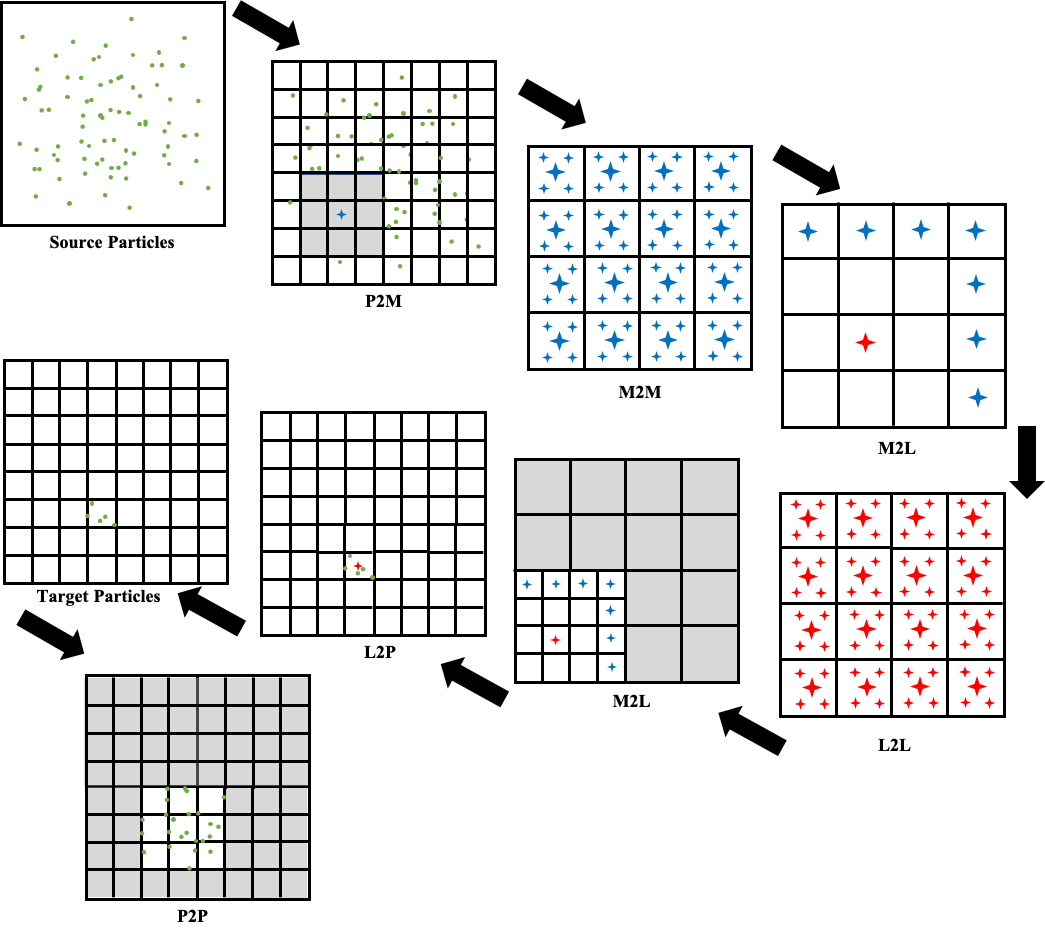
\includegraphics[width=1.1\textwidth]{introduction/main_loop.png}}
  \caption{
      The main FMM loop in two dimensions, encapsulating the upward and downward
      pass. The same set of particles are used for the sources and targets, and
      are shown in green. Local expansions are illustrated with red stars, and
      multipole expansions are illustrated with blue stars. For the P2M step the
      grey region indicates the \gls{near-field}, where this multipole expansion
      does not converge. For the M2L and P2P steps the grey region indicates
      box interactions already compressed and available via the translation or
      direct usage of local expansions. The larger/smaller stars in the M2M and
      L2L steps correspond to the parent/child expansions.
  }
  \label{fig:1_1_main_loop}
\end{figure}

\subsection{Summary}

The main practical challenge in implementing software to solve the analytic FMM
is the requirement of kernel-specific code to calculate the expansion coefficients of
(\ref{eq:1_1_multipole_expansion}) and (\ref{eq:1_1_local_expansion}). For example,
multiple different implementations already exist for Poison problems alone \cite{Greengard:1996:JCP, Etheridge:2001:SIAM}.
In software engineering terms this is inconvenient for the purposes of studying
the applications of the FMM in multiple different problem settings, as it leads to the requirement
to implement problem-specific solvers for each kernel one may encounter. This
leads to a productivity overhead in either designing a single, extensible
library, which by definition will be complex to design. Or to otherwise
maintain multiple problem-specific libraries.

The algorithm thus far described referred to as the analytic FMM is more correctly
called the non-adaptive analytic FMM. The non-adaptivity refers to the assumption that
all boxes at the leaf level are refined to the same degree, however as mentioned
in the above analysis of the algorithm, the degree of refinement is chosen such
that the number of particles in a leaf box is \textit{constant}. Therefore, If
the distribution of the particles of interest is not uniform over the computational
domain, one may be needlessly refining the boxes in some regions which may even be
empty. Therefore, although the asymptotic complexity of
the FMM is $O(N)$, it is clear that practical implementations will suffer unless
care is taken to use efficient vectorised data structures for the creation of
appropriate hierarchical tree required by the algorithm.

Additionally, there is significant scope for multiple levels of
parallelism in practical implementations. For example, the computations
for the local and multipole coefficients as well as the application of M2L, L2L
and M2M operators at a given level, are candidates for an implementation of
\textbf{\gls{task-level-parallelism}}. In addition to parallelising of each operator
application as a task, there is scope for implementing
\textbf{\gls{data-level-parallelism}} to find the expansion coefficients. For example,
Yokota and Barba \cite{Hwu:2011:MKP} demonstrate how the calculation of the P2P,
and M2L operators can be transferred to \textbf{\gls{GPU}}s using \textbf{\gls{CUDA}}.
The M2L, and P2P operators represent the largest computational bottlenecks due to
the number of such interactions in the FMM algorithm, therefore are a priority for
acceleration. For example, in three dimensions each target box has potentially
up to 189 source boxes in its \gls{interaction-list} with which to compute the
M2L operation, and for any particularly deep tree there will be roughly $O(N)$
leaf boxes, for which interactions are calculated directly. This leads to both of
these operations dominating the run-time of any \gls{FMM} implementation.

In summary, the implementation of the analytical FMM is complicated by the
fact that it is problem specific - which will also apply to any parallel
optimisation code. This in itself provides the main motivation for developing
an implementation that does not rely on explicit kernel expansions. Furthermore,
the desire for developer productivity, at the expense of hyper-optimised
implementations, is realised in this thesis by making use of Python,
a \textbf{\gls{high-level-interpreted-language}}, for our software implementation.
